% !TEX program = xelatex
\documentclass[11pt]{ctexart}
\usepackage[a4paper, margin=2.5cm]{geometry}
\usepackage{graphicx}
\usepackage{amsmath}
\usepackage{listings}
\usepackage{xcolor}
\usepackage{hyperref}

% ======== 个人信息（待填写） ========
\newcommand{\StudentName}{唐泽楠}
\newcommand{\StudentID}{24307140056}
% ===================================

\lstset{
  basicstyle=\ttfamily\small,
  language=C,
  keywordstyle=\color{blue!70!black},
  commentstyle=\color{green!45!black},
  columns=flexible,
  breaklines=true,
  frame=single,
  framerule=0.3pt,
  xleftmargin=0.5em,
  aboveskip=0.6em,
  belowskip=0.6em
}

\title{\textbf{Lab1：DataLab 实验报告}}
\author{\StudentName \quad \StudentID}
\date{\today}

\begin{document}
\maketitle

\section{测试结果}

\subsection{规则检查（\texttt{./check\_ops.py bits.c}）}

\begin{center}
  \IfFileExists{images/check_ops.png}{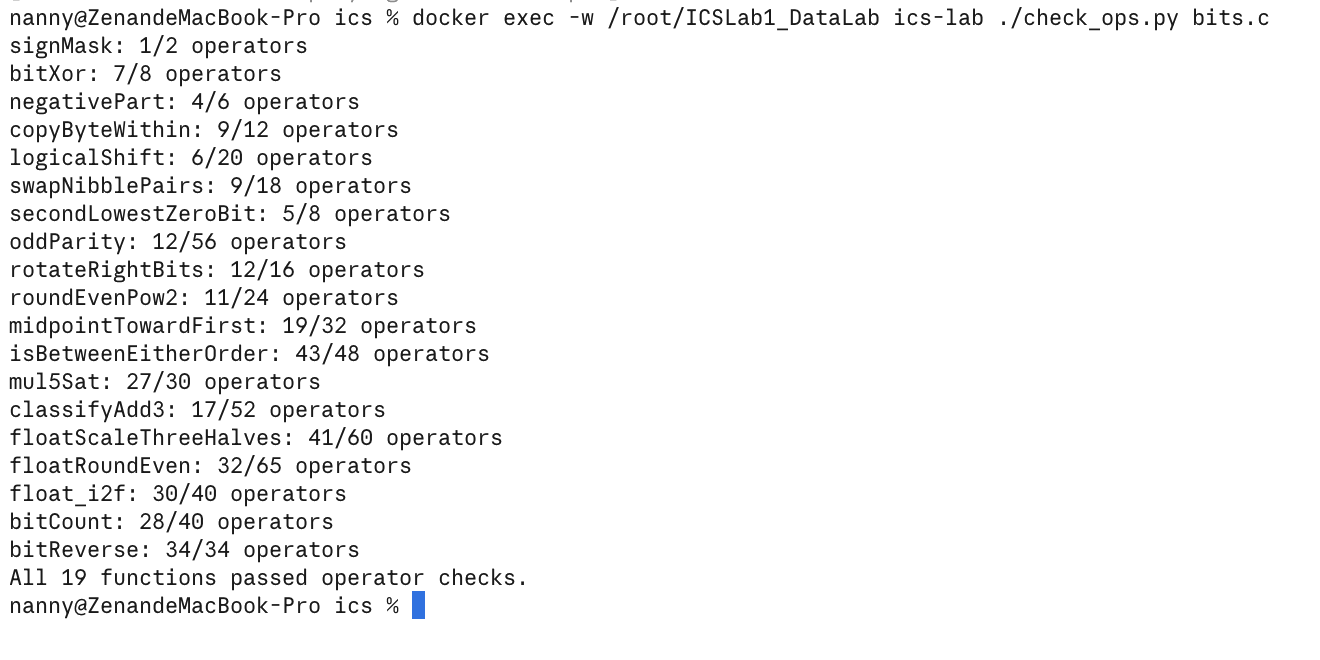
\includegraphics[width=0.85\textwidth]{images/check_ops.png}}{[截图占位：check\_ops]}
\end{center}

\subsection{正确性测试（\texttt{./btest}）}

\begin{center}
  \IfFileExists{images/btest.png}{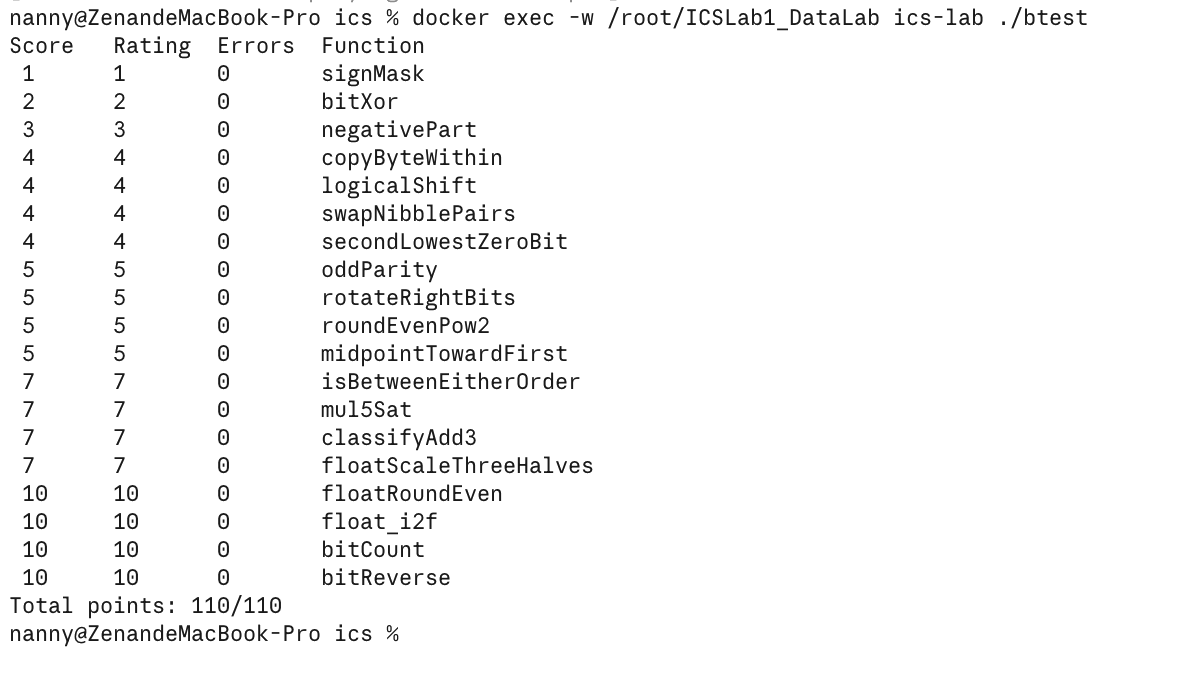
\includegraphics[width=0.85\textwidth]{images/btest.png}}{[截图占位：btest]}
\end{center}

全部 19 题通过规则检查，\texttt{btest} 得分 $110/110$。

\section{各函数实现思路}

\subsection{P1 \ signMask（2 ops 上限，实际 1 op）}
把 1 左移到符号位即可：\lstinline|return 1 << 31;|。左移进入符号位在本实验的
32 位位向量模型（\texttt{-fwrapv}）下是良定义的。

\subsection{P2 \ bitXor（仅 \texttt{\~{}} 与 \texttt{\&}，8 ops 上限，实际 7 ops）}
由布尔代数 $x \oplus y = (x \lor y) \land \lnot(x \land y)$，再用德摩根律把
$\lor$ 改写为 $\lnot(\lnot x \land \lnot y)$，得
\lstinline|~(~x & ~y) & ~(x & y)|。

\subsection{P3 \ negativePart（6 ops 上限，实际 4 ops）}
$x \gg 31$（算术右移）在 $x<0$ 时是全 1 掩码、否则为 0；补码取负 $-x=\lnot x+1$。
两者按位与：\lstinline|(~x + 1) & (x >> 31)|。$x=\mathit{INT\_MIN}$ 时
$-x$ 回绕为 $\mathit{INT\_MIN}$，与参考实现在 \texttt{-fwrapv} 下的行为一致。

\subsection{P4 \ copyByteWithin（12 ops 上限，实际 9 ops）}
字节号乘 8 用左移 3 位实现。先取出源字节
\lstinline|(x >> (src<<3)) & 0xFF|，再用掩码 \lstinline|0xFF << (dst<<3)|
清空目标字节，最后把源字节移位后或进去。

\subsection{P5 \ logicalShift（20 ops 上限，实际 6 ops）}
先做算术右移 \lstinline|x >> n|，再清除被复制进来的 $n$ 个符号位。
关键是构造``高 $n$ 位全 1''的掩码且对 $n=0$ 也成立：
\lstinline|((1 << 31) >> n) << 1| 算术右移得到高 $n{+}1$ 位为 1，再左移 1 位
恰好剩高 $n$ 位（$n=0$ 时 $0x80000000 \ll 1 = 0$）。取反后与结果相与。

\subsection{P6 \ swapNibblePairs（18 ops 上限，实际 9 ops）}
用常量拼出掩码 $m=\texttt{0x0F0F0F0F}$（每字节低 4 位）。
高低半字节互换即 \lstinline!((x >> 4) & m) | ((x & m) << 4)!：
右移后与 $m$ 相与同时清掉了算术移位带来的符号位污染。

\subsection{P7 \ secondLowestZeroBit（8 ops 上限，实际 5 ops）}
经典技巧：$y = x \,\vert\, (x+1)$ 把 $x$ 最低的 0 位填成 1；
而``最低 0 位''的掩码是 $\lnot y \,\&\, (y+1)$。于是第二低的 0 位
就是 $y$ 的最低 0 位。无第二个 0 位时（如 $-1$、\texttt{0x7FFFFFFF}），
$y+1$ 回绕后结果自然为 0。

\subsection{P8 \ oddParity（56 ops 上限，实际 12 ops）}
折半异或：依次 \lstinline|x ^= x>>16, x>>8, x>>4, x>>2, x>>1| 后，
bit0 即全部 32 位的异或（1 的个数的奇偶性）。个数为偶数时应返回 1，
故返回 \lstinline|(x & 1) ^ 1|。

\subsection{P9 \ rotateRightBits（16 ops 上限，实际 12 ops）}
实际旋转位数 $m = n \,\&\, 31$。结果为``$x$ 逻辑右移 $m$ 位''与
``$x$ 左移 $(32-m) \bmod 32$ 位''之或。逻辑右移复用 P5 的掩码技巧；
$(32-m) \bmod 32$ 用 \lstinline|(~m + 1) & 31| 实现（即 $-m \bmod 32$），
对 $m=0$ 两部分都退化为 $x$，结果正确。

\subsection{P10 \ roundEvenPow2（24 ops 上限，实际 11 ops）}
向偶数舍入的``加偏置再截断''技巧：设 $\mathit{half}=2^{n-1}$，偏置
$\mathit{bias} = \mathit{half} - 1 + q_0$，其中 $q_0$ 是商 $\lfloor x/2^n\rfloor$
的最低位。则 \lstinline|((x + bias) >> n) << n| 恰好实现四舍六入五留双：
余数 $<\mathit{half}$ 时加偏置不进位（向下）；余数 $>\mathit{half}$ 时必进位（向上）；
余数恰为 $\mathit{half}$ 时是否进位由 $q_0$ 决定，商为奇数才进位，从而商总被舍到偶数。
$-1$ 用 $\lnot 0$ 构造，$2^{n-1}$ 用 \lstinline|1 << (n + ~0)| 构造。
由于 $x \le \texttt{0x3fffffff}$、$n \le 16$，加法不会溢出。

\subsection{P11 \ midpointTowardFirst（32 ops 上限，实际 19 ops）}
无溢出取平均的恒等式：$x+y = 2(x\&y) + (x\oplus y)$，故
$\lfloor (x+y)/2 \rfloor = (x\&y) + ((x\oplus y) \gg 1)$（算术右移即向下取整除 2，
对负数同样成立）。当和为奇数（$(x\oplus y)\&1=1$）且 $x>y$ 时，中点应向 $x$ 取整，
即再加 1。比较 $x>y$ 需防溢出：符号相同时看 $y-x$ 的符号位（此时减法不会溢出），
符号不同时 $x>y$ 当且仅当 $y<0$。

\subsection{P12 \ isBetweenEitherOrder（48 ops 上限，实际 39 ops）}
结果为 $(a\le x \land x\le b) \lor (b\le x \land x\le a)$。实现一个防溢出的
$p\le q$ 判定（结果为全 1 / 全 0 掩码）：符号不同时 $p\le q \iff p<0$；
符号相同时 $q-p$ 不会溢出，$p\le q \iff (q-p)$ 符号位为 0。
四次比较共享三个符号位和两个符号差异标志；$a-x$、$x-b$ 直接由
$x-a$、$b-x$ 取负得到（同号时 $x-a \ne \mathit{INT\_MIN}$，取负精确），
每个只花 2 ops。最后按逻辑组合并 \lstinline|& 1| 得 0/1。

\subsection{P13 \ mul5Sat（30 ops 上限，实际 27 ops）}
$5x$ 不溢出当且仅当 $-c \le x \le c$，$c = \lfloor \mathit{INT\_MAX}/5\rfloor
= \texttt{0x19999999}$（可验证 $x=c$ 时 $5c = 2^{31}-3$ 恰好不溢，
$x=-c-1$ 时恰好下溢）。$c$ 由 0x19、0x99 移位拼出。
上溢判定 $x>c$ 只在 $x\ge 0$ 时可能：此时 $c-x$ 不会溢出，看其符号位，
并用 $\lnot(x\gg 31)$ 做符号门控；下溢判定 $x<-c$ 同理只在 $x<0$ 时用
$x+c$ 的符号位。乘积本身用 \lstinline|(x << 2) + x| 计算低 32 位，最后
按三个互斥掩码从 $\{ \texttt{0x7FFFFFFF},\ \texttt{0x80000000},\ 5x \}$ 中选择。

\subsection{P14 \ classifyAdd3（52 ops 上限，实际 17 ops）}
设 $w = x + y$（回绕）、$t = w + z$（回绕）。每次补码加法与数学真值的差恰为
$k\cdot 2^{32}$，$k\in\{-1,0,1\}$：正溢出时 $k=+1$，负溢出时 $k=-1$。
溢出发生当且仅当两操作数同号且与结果异号，即
$((x\oplus w)\,\&\,(y\oplus w))$ 的符号位为 1；溢出方向由操作数符号给出，
用 \lstinline!(x>>31) | 1! 得到 $\pm 1$。于是真和 $= t + (k_1+k_2)\cdot 2^{32}$。
关键观察：$k_1 = +1$ 蕴含 $w<0$，而第二次正溢出要求 $w\ge 0$，故 $k_1,k_2$
不可能同为 $+1$（同为 $-1$ 对称），$K=k_1+k_2 \in \{-1,0,1\}$。
又 $t\in[\mathit{INT\_MIN},\mathit{INT\_MAX}]$，故真和越上界 $\iff K=1$、
越下界 $\iff K=-1$、否则 $K=0$ —— $K$ 本身就是要求的返回值，直接返回 $k_1+k_2$。

\subsection{P15 \ floatScaleThreeHalves（60 ops 上限，实际约 41 ops）}
拆出符号、阶码、尾数三段后分类：
\begin{itemize}
  \item $\mathit{exp}=255$：NaN 或无穷，直接返回 \texttt{uf}（无穷乘 1.5 仍为同号无穷）。
  \item $\mathit{exp}=0$（非规格化）：编码的量值域是线性的，直接令 $m=3\cdot
    \mathit{frac}$ 再除 2 并向偶舍入（丢弃位为 1 时恰是中点，结果为奇则加 1）。
    若结果进位到 bit23，编码上自然变成 $\mathit{exp}=1$ 的规格化数，无需特判。
  \item 规格化：$M = 2^{23}+\mathit{frac}$，$m = 3M \in [3\cdot 2^{23},\, 3\cdot 2^{24})$，
    目标值为 $m\cdot 2^{\mathit{exp}-151}$。若 $m < 2^{25}$，尾数取 $m/2$、阶码不变，
    对丢弃的 1 位向偶舍入；否则尾数取 $m/4$、阶码加 1，对丢弃的 2 位按
    $r=1$ 舍、$r=3$ 入、$r=2$ 向偶处理。舍入进位到 $2^{24}$ 时再右移一位并阶码加 1。
    阶码达到 255 时返回同号无穷（此时真值 $\ge 2^{128}$，向最近舍入必为无穷）。
\end{itemize}

\subsection{P16 \ floatRoundEven（65 ops 上限，实际约 32 ops）}
按指数分段：
\begin{itemize}
  \item $\mathit{exp}=255$：NaN/无穷，原样返回。
  \item $\mathit{exp}\le 125$（含非规格化）：$|f|<0.5$，舍入到 $\pm 0$，返回符号位。
  \item $\mathit{exp}=126$：$|f|\in[0.5,1)$。恰为 0.5（尾数为 0）时向偶舍入到 $\pm 0$；
    否则舍入到 $\pm 1$（返回 \lstinline!sign | 0x3F800000!）。
  \item $\mathit{exp}\ge 150$：$2^{23}$ 的整数倍刻度以上本身就是整数，原样返回。
  \item 其余（$1\le |f| < 2^{23}$）：设 $k = 150-\mathit{exp}$ 为小数位数，
    对 $M=2^{23}+\mathit{frac}$ 的低 $k$ 位做标准的向偶舍入
    （低位 $>$ 半值进位；恰为半值时整数部分为奇才进位），
    再左移 $k$ 位放回。进位越过 bit23 时右移一位并阶码加 1（此时低位全 0，无精度损失）。
\end{itemize}

\subsection{P17 \ float\_i2f（40 ops 上限，实际约 30 ops）}
$x=0$ 特判返回 0。否则记录符号并取绝对值（$x=\mathit{INT\_MIN}$ 时
\lstinline|-x| 回绕为 \texttt{0x80000000}，作为无符号数恰是正确的绝对值）。
用 while 循环找最高位 $h$，阶码为 $h+127$。若 $h\le 23$，尾数左移补齐即可精确表示；
否则需丢弃低 $h-23$ 位，按``大于半值进位、等于半值向偶''舍入，
舍入进位溢出到 bit24 时右移一位并阶码加 1。最后拼接符号、阶码与去掉隐含 1 的尾数。

\subsection{P18 \ bitCount（40 ops 上限，实际 28 ops）}
经典分治 popcount。用 \texttt{0x55}、\texttt{0x33}、\texttt{0x0F} 拼出
32 位掩码 \texttt{0x55555555}、\texttt{0x33333333}、\texttt{0x0F0F0F0F}，
依次做 1 位、2 位、4 位分组求和；4 位分组后每字节的计数至多 8，
后续 \lstinline|x + (x>>8)|、\lstinline|x + (x>>16)| 不会跨组进位，
最后 \lstinline|& 0x3F| 取出总数。

\subsection{P19 \ bitReverse（34 ops 上限，实际 34 ops）}
标准的对折反转：依次交换 16 位半字、8 位字节、4 位半字节、2 位对、相邻位。
操作数上限较紧，掩码用递推构造节省操作：
\lstinline!m16 = 0xFF | (0xFF<<8)! 得 \texttt{0x0000FFFF}，之后每个掩码由
$m' = m \oplus (m \ll w)$ 得到（\texttt{0x00FF00FF}、\texttt{0x0F0F0F0F}、
\texttt{0x33333333}、\texttt{0x55555555}），每个仅 2 ops。
半字交换中 \lstinline|(x >> 16) & m16| 同时完成了逻辑右移。
总操作数恰为 34，等于上限。

\section{参考资料}
\begin{itemize}
  \item Randal E. Bryant, David R. O'Hallaron. \emph{Computer Systems: A Programmer's Perspective (3rd Edition)}, 第 2 章（整数与浮点数表示）。
  \item Henry S. Warren, Jr. \emph{Hacker's Delight (2nd Edition)}：无溢出求平均值 $(x\&y)+((x\oplus y)\gg 1)$、分治 popcount、位反转、最低 0 位掩码等经典位技巧。
  \item IEEE 754-2008 单精度浮点格式与 round-to-nearest-even 舍入规则。
\end{itemize}

\end{document}
